\documentclass{article}
\usepackage[utf8]{inputenc}

\title{Strong capacitive interactions within the non-equilibrium Green's Function Formalism.}
\author{Josko de Boer \and Jose Celis Gil \and Jos Seldenthuis \and Jos Thijssen}
\date{December 2016}
\usepackage[square,numbers]{natbib}
\bibliographystyle{abbrvnat}
\usepackage{fourier}
\usepackage{multicol}
\usepackage{fullpage}
\usepackage[british]{babel} 
\usepackage{mathrsfs}
\usepackage{amsthm,amsmath,amssymb,amsfonts}  
\usepackage{braket} 
\usepackage{subcaption}
\usepackage{xcolor}
\usepackage{graphicx}
\renewcommand{\thefootnote}{\Roman{footnote}}
\newcommand{\red}[1]{ {\color{red} #1}}
\date{February 2017}

\begin{document}
\maketitle
\begin{abstract}
    Most work on interactions for molecular junctions have been performed within the Master equation approach. This approach has the benefit of incorporating vibrational excitations and interactions up to desired order. In this work we focus on the non-equilibrium Green's function formalism. We incorporate interactions and derive the many-body Green's function. The density matrix emerges as a simple equation using the self-energy. We first apply these principles to the case of a Coulomb Island, a much studied and discussed nanoscopic device.  Having established both the basics and the Kondo physics of this device, we move on to consider the intrinsic and pronounced Negative Differential Conductance NDC effect in a single thiolated arylethynylene molecule with a 9,10-dihydroanthracene. We show that incorporation of strong capacitive interaction greatly improves the agreement between theory and experiment. The new theory has exciting promise for future studies of molecular junctions.
\end{abstract}
\begin{multicols}{2}
        
    \section{Introduction}
        A very common issue in the area of molecular electronics is the difficulty to find quantitative agreement between the theory and the experiments. This makes the design and prediction of functioning electronic devices based on molecules harder.
        
        Part of this issue is due to the difficulty to to incorporate all the details of specific molecules in the description of molecular junctions. Many-body techniques, with a single-particle picture are often used to describe these systems \cite{Tsuneda2014}. One of the most popular methods used nowadays consists of an approach where the electronic orbitals are solutions of a Schr\"odinger equation that depends on the electron density. This approach, called density functional theory (DFT), is the result of Hohenberg, Kohn and Sham work \cite{Hohenberg1964, kohnsham, nobel1998} and has proven to be a highly competitive method for a wide range of applications.
        
        When a molecule is coupled to metallic electrodes and a bias voltage is applied over the molecule which causes current to flow, then the system does not have a well-defined ground state. For such a system, trying to solve the Schr\"odinger equation directly is unfeasible. Non-equilibrium Green's Functions (NEGF) methods provide a systematic approach to incorporate interactions with an infinitely large environment including bias. NEGF are regularly used to calculate current and charge densities in non-equilibrium many-body transport problems \cite{Mattuck1976, Jauho1994, Haug1997, Datta1997}. 
         
        %One popular approach to solve the Kohnn-Sham equations \cite{kohnsham}, which reformulate the many-body Schr\"odinger equation in terms of the electron density $n(\underline{r})=\sum_{\sigma,i}\:n_{\sigma i}(r)$. This is called Density-Functional theory (DFT) \cite{nobel1998}, which leads to the single-particle Hamiltonian of a specific molecule.  
                
        If the transport properties of a system are affected by its vibrational modes, the NEGF equations tend to become unwieldy and computationally expensive as all many-body interactions on the molecule are taken into account explicitly. Theoretically, this obstacle in calculations is bypassed making use of the master equation (ME) approach \cite{beenakker}, which is a considerable simplification, yet it retains the many-body character of the system. However, both approaches ME and NEGF struggle with accounting for strong interactions.
        
        In some sense the NEGF and the ME approaches are opposite, while the starting point on the ME approach is an entire set of many-body states and their transitions, in the NEGF approach the starting point is a set of single-particle states and a Hamiltonian that describes the interactions between them, but despite the initial difference, it can be shown that ME can be derived from NEGF.
            
        In the present paper, we present a method, where making use of the NEGF approach, we incorporate strong capacitive interactions \emph{capactive} in molecular junctions. This method makes emphasis in the many-body character of the system and results in a better agreement between theory and experiments.
        
        In section~\ref{sec:derivation}, we derive and introduce the theory behind our method and in section~\ref{sec:island} we illustrate its effectiveness and completeness by mean of the Coulomb Island model. For a far more interesting example, in section~\ref{sec:ahmolecule} we look at the Negative Differential Conductance (NDC) found by Perrin et. al. \cite{perrinnano} in a single thiolated arylethynylene molecule (AH molecule) with a 9,10-dihydroanthracene core, where the theoretical and experimental current have been found to match qualitatively but not quantitatively. Finally, we discuss the findings of our theory and its future promises in section~\ref{sec:discussion}.


    
    \section{Derivation}\label{sec:derivation}
        Let us start with defining a generalised Anderson model for a central region with energy spectrum $\epsilon_i$ (operators $\hat{d_i}, \hat{d_i}^\dagger$) coupled to leads (operators $\hat{c}_k, \hat{c}_k^\dagger$):
        \begin{align}
            H &= H_1 + H_2 + H_\tau + H_\text{ML} + H', \label{eq:hamiltonian}
        \end{align}
        where
        \begin{align*}
        H_1 &= \sum_i \epsilon_i \hat{d_i}^\dagger \hat{d_i}, \\
        H_2 &= \sum_k E_k \hat{c_k}^\dagger \hat{c_k}, \\
        H_\tau &= \sum_{ij} \tau_{ij} \hat{d}_i^\dagger \hat{d}_j, \\
        H_\text{CL} &= \sum_{ki}\left\{ V_{ki} \hat{c_k}^\dagger \hat{d_i} +  V_{ki}^\dagger \hat{d_i}^\dagger \hat{c_k} \right\},\\
        H' &= \frac{1}{2} \sum_{ij} U_{ij} \hat{d_i}^\dagger \hat{d_i}\hat{d_j}^\dagger \hat{d_j}.
        \end{align*}
        $H_1$ describes the central region, $H_2$ describes the fermion bath, $H_\tau$ describes tunnelling in the central region, $H_\text{CL}$ describes coupling of the central region to the leads and $H'$ describes interaction between states in the central region. Modelled in this way the central region can be anything, but in the current discussion it will usually be a molecule.
    
        To find the Green's Function $G(t,t')$ we use the equation-of-motion method. The definition of the (retarded) Green's function is:
       \begin{align*}
        G_{ij}^+ &= - \frac{\imath}{\hbar} \theta(t-t^\prime) \left\{ \hat{d}_i(t), \hat{d}_j^\dagger(t^\prime) \right\},
        \end{align*}
        so that the full time derivative takes the form:
        \begin{align}
        \imath\hbar \dot{G}_{ij}^+ &= \delta_{ij} \delta(t - t^\prime) + \theta(t-t^\prime) \left\{ \dot{\hat{d}}_i (t), \hat{d}_j^\dagger (t')\right\},
        \label{eq:eomgf} 
        \end{align} where by substituting $\dot{\hat{d}}_i$ for the expression recovered from its Heisenberg equation of motion we find the expression for the Green's Function. To do so we need the commutators of the different terms with the creation operator $d^\dagger_i$:
        \begin{align*}
            \left[ \hat{d}_i, H_1 \right] &= \epsilon_i \hat{d}_i, \\
            \left[ \hat{d}_i, H_2 \right] &= 0, \\
            \left[ \hat{d}_i, H_\tau \right] &= \sum_j \tau_{ij} \hat{d}_k, \\
            \left[ \hat{d}_i, H_\text{CL} \right] &= \sum_k V_{ki} \hat{c}_k,\\
            \left[ \hat{d}_i, H' \right] &= \sum_l U_{il} \hat{n}_l \hat{d}_i,
        \end{align*}
        where the first four commutators are both well known and can be formulated as self-energies using the Dyson equation. The fourth commutator involves a annihilation operator working on the lead. However, it can be recovered as a self-energy by applying the EOM to find the lead-molecule Green's function $G_{kj}$, leading to the lead-molecule coupling self-energy $\Sigma^\pm$.        
        
        The last commutator still involves operators $\hat{n_l}$ and is not clearly a matrix product. By defining the capacitive self-energy: 
        \begin{align*}
        \hat{\Sigma}^C_{il} &= \sum_k U_{lk} \hat{n}_k \delta_{li},
        \end{align*}
        we have an expression that can be written as a matrix product, but still involves operators. This can be remedied by applying the following expansion of operators\red{[citation]}:
        \begin{align}
        \left[ \hat{A}^{-1} - \hat{B}\right]^{-1} &=\hat{A} + \hat{A}\hat{B}\hat{A} + \hat{A}\hat{B}\hat{A}\hat{B}\hat{A} + \ldots,
        \label{eq:expansion} \\
        &= \hat{A} \sum_n \left(\hat{B}\hat{A}\right)^n
        \end{align} 
        where we will attempt to recover a form similar to that found in \citet{haugjauho}, a sum of the contributions of different many-body states. The new object will be called the \emph{many-body} Green's function and be denoted by the symbol $\mathscr{G}$:
        \begin{align}
            \mathscr{\hat{G}}^\pm(\epsilon) &= \left[ \epsilon - \epsilon_i - \tau \pm \Sigma - \hat{\sigma^C}\right]^{-1}, \\
            &= \left[ \left(G^\pm\right)^{-1}- \hat{\Sigma^C}\right]^{-1} ,\nonumber
        \end{align}
        where $G^\pm$ denotes the Green's Function when capacitive interaction is not included. 
        
        
        We will first look at the example of a two-state model, where $\hat{\Sigma}^C = \begin{pmatrix} U_{12}n_2 & 0 \\ 0 & U_{21} n_1\end{pmatrix}=C^1 n_1 + C^2 n_2$. For the first few orders, we find:
        \begin{align*}
            \left(\mathscr{G}^\pm\right)^{(0)} &= (1-n_1)(1-n_2)G + n_1(1-n_2)G + (1-n_1) n_2 G \\&+ n_1 n_2 G,  
        \end{align*}
        \begin{align*}
            \left(\mathscr{G}^\pm\right)^{(1)} &=  n_1(1-n_2)GC^1 G + (1-n_1) n_2 G C^2 G +\\& n_1 n_2 G \left(C^1+C^2\right) G, \\
            \left(\mathscr{G}^\pm\right)^{(2)} &=  n_1(1-n_2)GC^1 GC^1 G + (1-n_1) n_2 G C^2 GC^2 G +\\& n_1 n_2 G \left(C^1+C^2\right) G\left(C^1+C^2\right) G, 
        \end{align*}
        where we clearly see a pattern:
        \begin{align*}
            \left(\mathscr{G}^\pm\right)^{(n)} &= \left[n_1 (1-n_2) \left(G C^1\right)^n + (1-n_1) n_2 \left(GC^2\right)^n\right. \\ & \left. + n_1 n_2 \left(G (C^1 +C^2)\right)^n\right] G \quad \forall n \geq 1,
        \end{align*}
        which can be proven by mathematical induction:
        \begin{align*}
        \left(\mathscr{G}^\pm\right)^{(n+1)} &= \left( G (C^1 n_1 + C^2 n_2\right)^{n+1} G \\
        &= G (C^1 n_1 + C^2 n_2 )\left(\mathscr{G}^\pm\right)^{(n)} \\
        &= \left[ n_1 (1-n_2) G C^1 (GC^1)^n \right. \\ &+ (1-n_1) n_2 G C^2(GC^2)^n \\ &+ n_1 n_2 GC^1 (G (C^1+C^2))^n \\ &\left.+ n_1 n_2 GC^2 (G (C^1+C^2))^n \right] G
        \end{align*}
        
        Gathering terms for the two-state model and applying equation~\ref{eq:expansion} reversely, we find the exact expression:
        \begin{align}\label{eq:mbgf2}
            \mathscr{G}^\pm &= (1-n_1)(1-n_2) G \\ &+ n_1 (1-n_2) \left[ G^{-1} - U_{12}\right]^{-1} \nonumber\\ &+ (1-n_1)n_2 \left[ G^{-1} - U_{21}\right]^{-1} \nonumber\\ &+ n_1 n_2\left[ G^{-1} - U_{21} - U_{12}\right]^{-1} \nonumber,
        \end{align}
        in general, the expression becomes:
        \begin{align}\label{eq:mbgf}
        \mathscr{G}^\pm &= \sum_\kappa \left(\prod_{i\in\kappa} n_i \prod_{j\notin \kappa} (1-n_j) \right) \left[G^{-1} - \sum_{i\in\kappa} \sum_{j\notin \kappa} U_{ij}\right]^{-1}m \\
        \nonumber &= \sum_\kappa \left(\prod_{i\in\kappa} n_i \prod_{j\notin \kappa} (1-n_j) \right) G^{\kappa\pm},
        \end{align}
        where $G^{\kappa\pm}$ is a shorthand. Clearly, the expectation value is just $\mathscr{G} = \sum_\kappa \left|C_\kappa\right|^2 G^{\kappa}$. This is the sought-after expansion in the contributions of the different many-body states.
                  
        Nevertheless, we still have to consider the problem of determining the expectation values of number operators. First, recall the single-particle state occupation numbers:
        \begin{align*}
            \braket{\hat{n}_i} &= \sum_{\kappa: i\in \kappa} P_{\kappa\kappa},
        \end{align*}
        where the sum is over those many-body states $\ket{\kappa}=\left(\prod_{i\in\kappa}\hat{d}_i^\dagger \right)\ket{0}$ in which the single-particle state $\ket{i} = \hat{d}_i^\dagger \ket{0}$ is occupied. We can represent the the vector of occupation numbers by a matrix equation $\braket{\underline{n}} = KP$, where $P=\text{diag}(P_{\kappa\kappa})$ and $K$ is defined by:
        \begin{align}
            K_{i\beta} = \begin{cases} 1 & \quad i\&B=i, \\ 0 & \quad\text{otherwise}\end{cases},
        \label{eq:kmatrix}\end{align}
        where $\&$ is the binary \emph{and} operator.
        
        We can also find $\braket{n_i}$ via the lesser Green's function:
        \begin{align*}
            \braket{n_i} &= \lim_{t\rightarrow t'} \frac{\hbar}{\imath} \braket{\mathscr{G}^<_{ii}(t-t')}, \\
            &= \sum_\kappa \left|C_\kappa\right|^2 \int \frac{d\epsilon}{2 \pi \imath} G^{\kappa<}, \\
            &= \sum_\kappa \left|C_\kappa\right|^2 \int \frac{d\epsilon}{2 \pi} \left[ \sum_\alpha f_\alpha(\epsilon) G^{\kappa+} \Gamma^\alpha G^{\kappa-}\right]_{ii},
        \end{align*}
        where the penultimate step utilises both the Keldysh equation \cite{diventra} and the Fluctuation-Dissipation theorem \cite{haugjauho}.      
         
        It is important to remember that the fluctuation-dissipation theorem specified the Fermi-Dirac distribution on the \emph{contacts}, thereby introducing finite bias as a relevant parameter for the density-matrix solution. We have found the following equations for $\braket{\underline{n}}$:
        \begin{align}
            \braket{\underline{n}} &= WP = KP\label{eq:selfconsistent},
        \end{align}
        where it cannot be guaranteed that the null-space of $W-K$ is one-dimensional. We could then use a self-consistent scheme to solve for $\braket{\underline{n}}$ starting from the equilibrium vector. This is conceptually similar to turning on the non-equilibrium interactions adiabatically, which could be interpreted as a variation of the Gell-Man-Low theorem\cite{gellmannlow, molinari}, yet is not because a self-consistent scheme cannot guarantee adiabatic steps.
        
        However, we must consider the implications of a null-space containing more than one vector. The physical quantity, $\braket{\underline{n}}$ is certainly unique. This implies that all vectors in the null-space result in the same value of the physical quantity. As a result, any vector in the null-space suffices to calculate the expectations of number occupation operators. This then immediately results in a unique green function which allows us to calculate transport properties of the equation.

    \section{The Coulomb Island}\label{sec:island}
        We are now ready to perform the calculations for a Coulomb Island. Following \citet{haugjauho}, we will set $\hat{H}_\tau = 0$. We need to be careful with the incorporation of the leads. In the penultimate step for equation~\ref{eq:wmatrix}, we note a summation over each lead due to the fluctuation-dissipation theorem. 
        
        For a two-state system (spin up, spin down) we find:
        \begin{align*}
            G^{\lambda<}_{ii}(\epsilon) &= \left(\left|G_{1i}(\epsilon)\right|^2 + \left|G_{i2}(\epsilon)\right|^2 \right)\left(f^L (\epsilon) \gamma^L+f^R (\epsilon) \gamma^R\right),
        \end{align*}
        where we have used that $(G^+)^\dagger=G^-$ and that the coupling is described by a diagonal matrix. Here, $\gamma^\alpha$ denotes the coupling strength to the left (right) contact $\alpha$.
        
        \begin{figure*}[b]
            \centering
            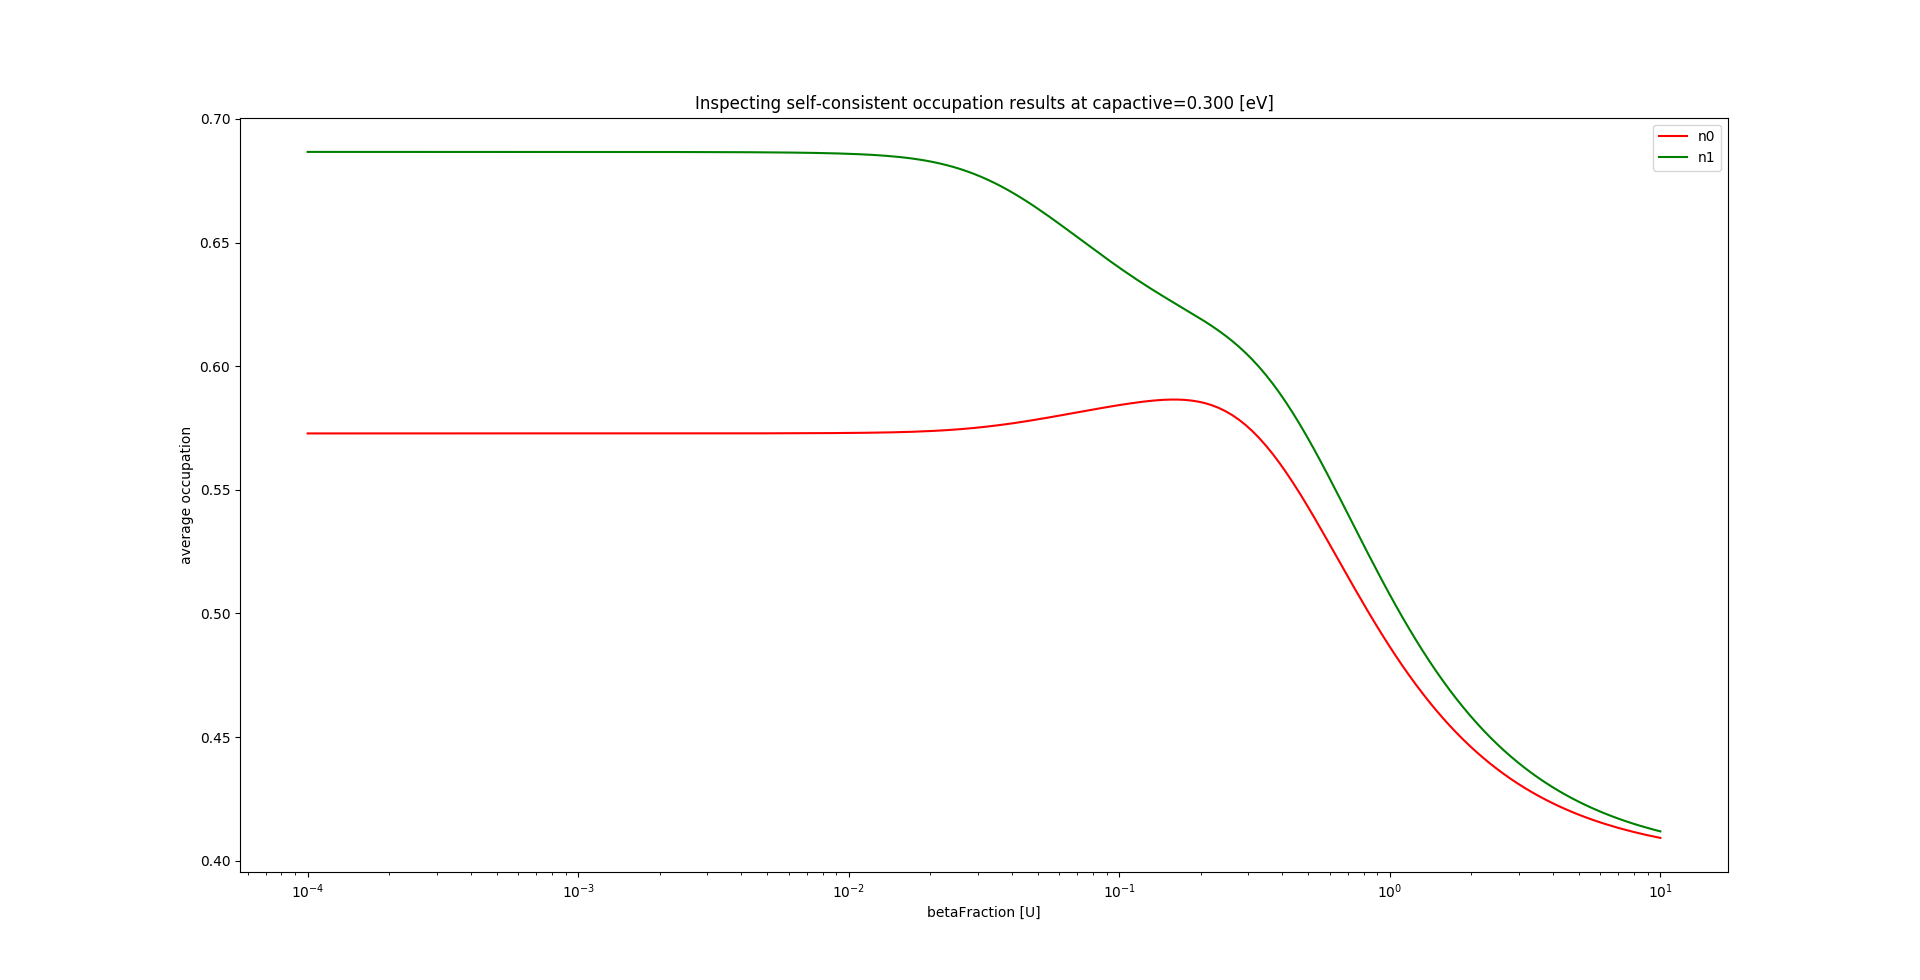
\includegraphics[width=\textwidth]{fig/figure_1.png}
            \caption{\label{fig:numberoperators}Expectation value of occupation number operators $n_1$ and $n_2$.The emergence of a bound state at low temperatures is evident.}
        \end{figure*}
         
        
        In our calculation, the lead-molecule coupling (WBL) $\gamma=.010$ eV, the Coulomb repulsion $U=0.300$ eV, the first level is at $0.00$ eV and the second level at $0.030$ eV. We can immediately calculate the expectations of number operators, shown in fig~\ref{fig:numberoperators}.We observe the emergence of a bound state at low temperatures, evident in the exponential growth of $n_1$. In stark contrast, $n_0$ reaches its maximum and then rapidly falls off. Considering that we are dealing with the exact calculation of occupation for an Anderson-model, it is likely that we are observing evidence of the Kondo effect \cite{josherrereview}. This is typically evident in the conductance $\sigma(T)$, which decreases as a Fermi-liquid (polynomial) until reaching a conductance minimum at the Kondo temperature $T_K$, after which it grows logarithmically until saturating because of low-temperature screening effects.
        
        Following \citet{meir}, we look primarily at the conductance $\mathscr{T}(\epsilon)$ versus the chemical potential $\epsilon$. In a non-equilibrium situation the Fermi energy is rather badly defined; even more so in a mesoscopic region. The Fermi energy is a bulk property of the Fermi liquid model which does not hold in the extended molecule region. As such, we will consider the full conductance spectrum and follow the conductance maximum.
        
        Fig~\ref{fig:transplot} displays the differential conductance $T(\epsilon)$. Note the four peaks that are evidence of interaction effects for our two-state model. The differential conductance traces are offset by the temperature for reasons of clarity. A clear transition to zero-occupation is evident as the temperature grows.
        
        \begin{figure*}[b]
            \centering
            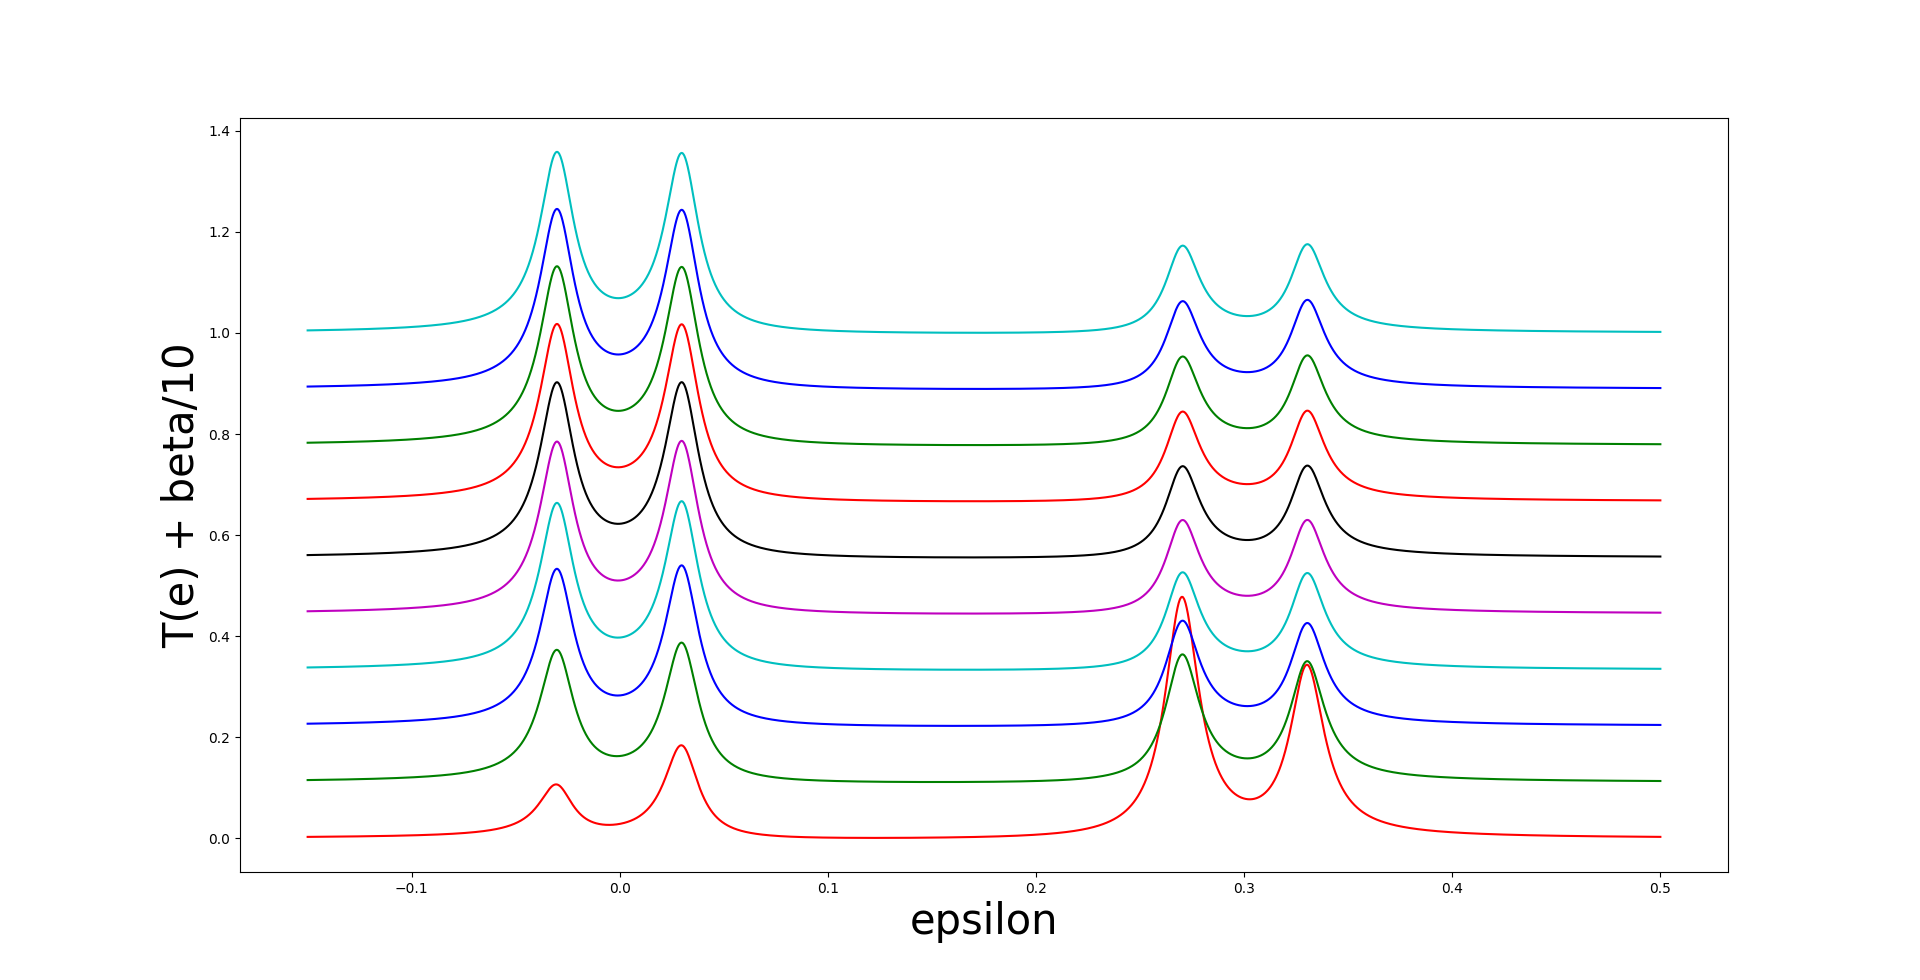
\includegraphics[width=\textwidth]{fig/figure_3.png}
            \caption{\label{fig:transplot} Differential conductance $T(\epsilon)$, displaying the multiple peaks that are evidence of interaction effects for our two-state model. The differential conductance traces are offset by the temperature for reasons of clarity. A clear transition to zero-occupation is evident as the temperature grows.}
        \end{figure*}
        
        This state is clearly the bound-state that is responsible for the Kondo effect. Fig~\ref{fig:conductance} shows the maximum conductance versus temperature, displaying clearly the polynomial decrease with temperature, followed by the conductance minimum, logarithmic rise and final screening saturation. It is interesting to note that there are two regions of the logarithmic rise before screening saturation, likely due to the different available levels.
        
        \begin{figure*}[b]
            \centering
            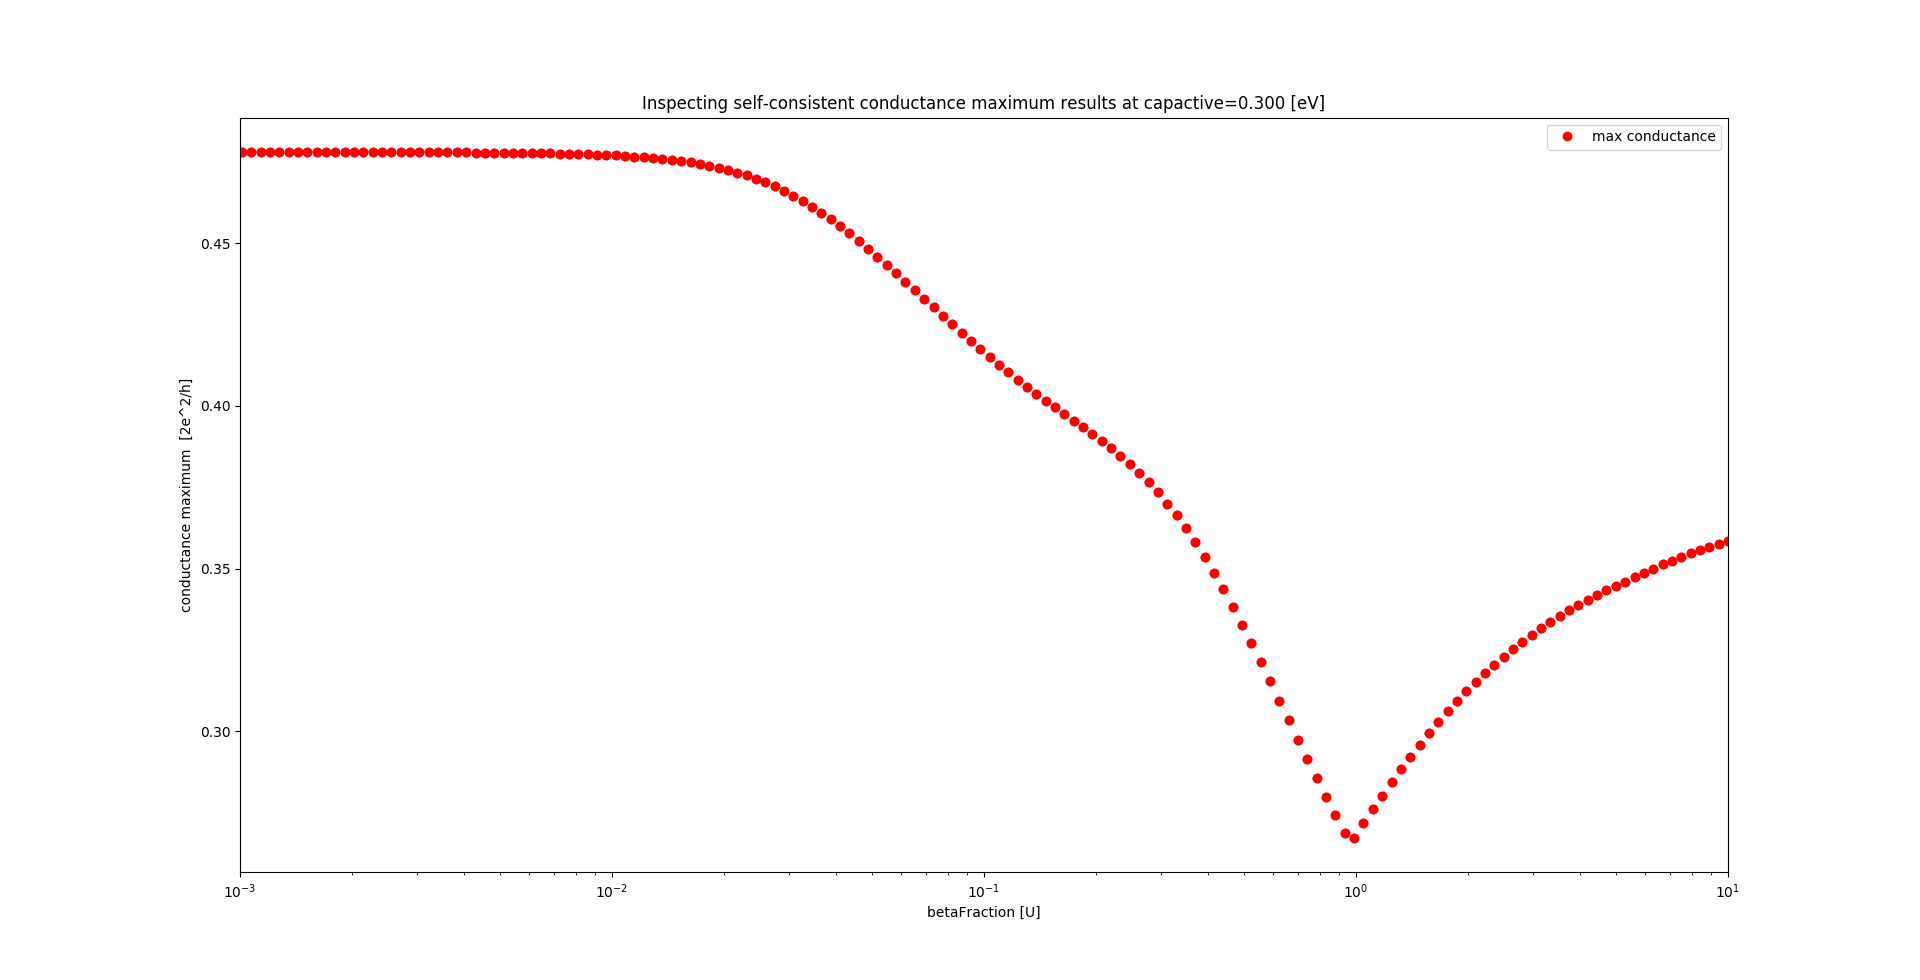
\includegraphics[width=\textwidth]{fig/figure_5.png}
            \caption{\label{fig:conductance} Average of the differential conductance versus temperature. The clear transition from Fermi liquid-like behaviour to logarithmic scaling is evident followed by saturation is evident.}
        \end{figure*}
        
        The maximum conductance plot of fig~\ref{fig:conductance} combined with the fractional charging indicates that the exact solution incorporates Kondo physics, contrary to many perturbation schemes that are often only valid away from the Kondo temperature $T_K$. Our exact solution thus does not suffer from difficulty in the crossover region. It shows excellent agreement with both theory and experiment \cite{Sasaki2000}. 
         
    \section{AH molecule}\label{sec:ahmolecule}
        
        The single thiolated arylethynylene (AH) molecule Negative Differential Conductance (NDC) was explained by a relatively simple two-site model with Stark effect in \citet{perrinnano}. Contrary to the Coulomb Island, there is tunnelling between the two levels. Only the 'left' level is coupled to the left electrode and the 'right' level is coupled to the right electrode. The full specification of the model is:
        \begin{align*}
            H_\text{AH} &= \begin{pmatrix} \epsilon_0 + \frac{1}{2}\alpha V & -\tau \\-\tau &  \epsilon_0 - \frac{1}{2} \alpha V\end{pmatrix}, \\
            \Gamma^L &= \begin{pmatrix} \gamma & 0 \\ 0 & 0 \end{pmatrix} ,\\
            \Gamma^R &= \begin{pmatrix} 0 & 0 \\ 0 & \gamma \end{pmatrix} ,\\
            H' &= \frac{1}{2} U \hat{n}_L \hat{n}_R + \frac{1}{2} U \hat{n}_R \hat{n}_L.
        \end{align*}
        The model is thus exactly of the class of models discussed above. The transport eigenvalues are $\epsilon_\pm = \epsilon_0 \pm \frac{1}{2} \sqrt{\alpha^2 V^2 + 4\tau^2}$ and we can expect peaks in current at $V = \pm \sqrt{ \frac{4\tau^2}{1-\alpha^2}}$, when the transport eigenvalue intersects the symmetrically distributed bias $\pm \frac{V}{2}$. Of course there is a second set of transport eigenvalues at $\epsilon_\pm + U$, which didn't feature in the experiment. However, a fractionally charged molecule might experience a coulomb blockade because of it.
        
        In figure~\ref{fig:perrinmolecule}, we display results for the AH molecule of \citet{perrinnano}. The green line in the top figure is the experimentally measured current from Perrin 's experiments averaged over a number of separation distances. The theoretical current is displayed with the same maximum current as the experiment, but the ratio is reported on top. It clearly reproduces the NDC effect, the location of the peaks and the flatness in between the two peaks. The peaks are also exactly located at the predicted value. The slope of the figure emphasises that fact. The occupancy of the two levels is clearly anti symmetric as expected from the properties of the system. Additionally, the occupancy shows a peak at the same location before saturating to $\braket{n_{L,R}}\approx0.5$.
    
        Strikingly, the difference in maximum current is within one order of magnitude for the new theory while \citet{perrinnano} reported a ratio of $1.4\cdot10^{4}$. However, the current drop off after reaching peak current is predicted significantly steeper than it was for \citet{perrinnano}.  {\color{red} which can be for many reasons (ie tunnelling etc)}.
        
        
        
    \begin{figure*}[b]
        \centering
        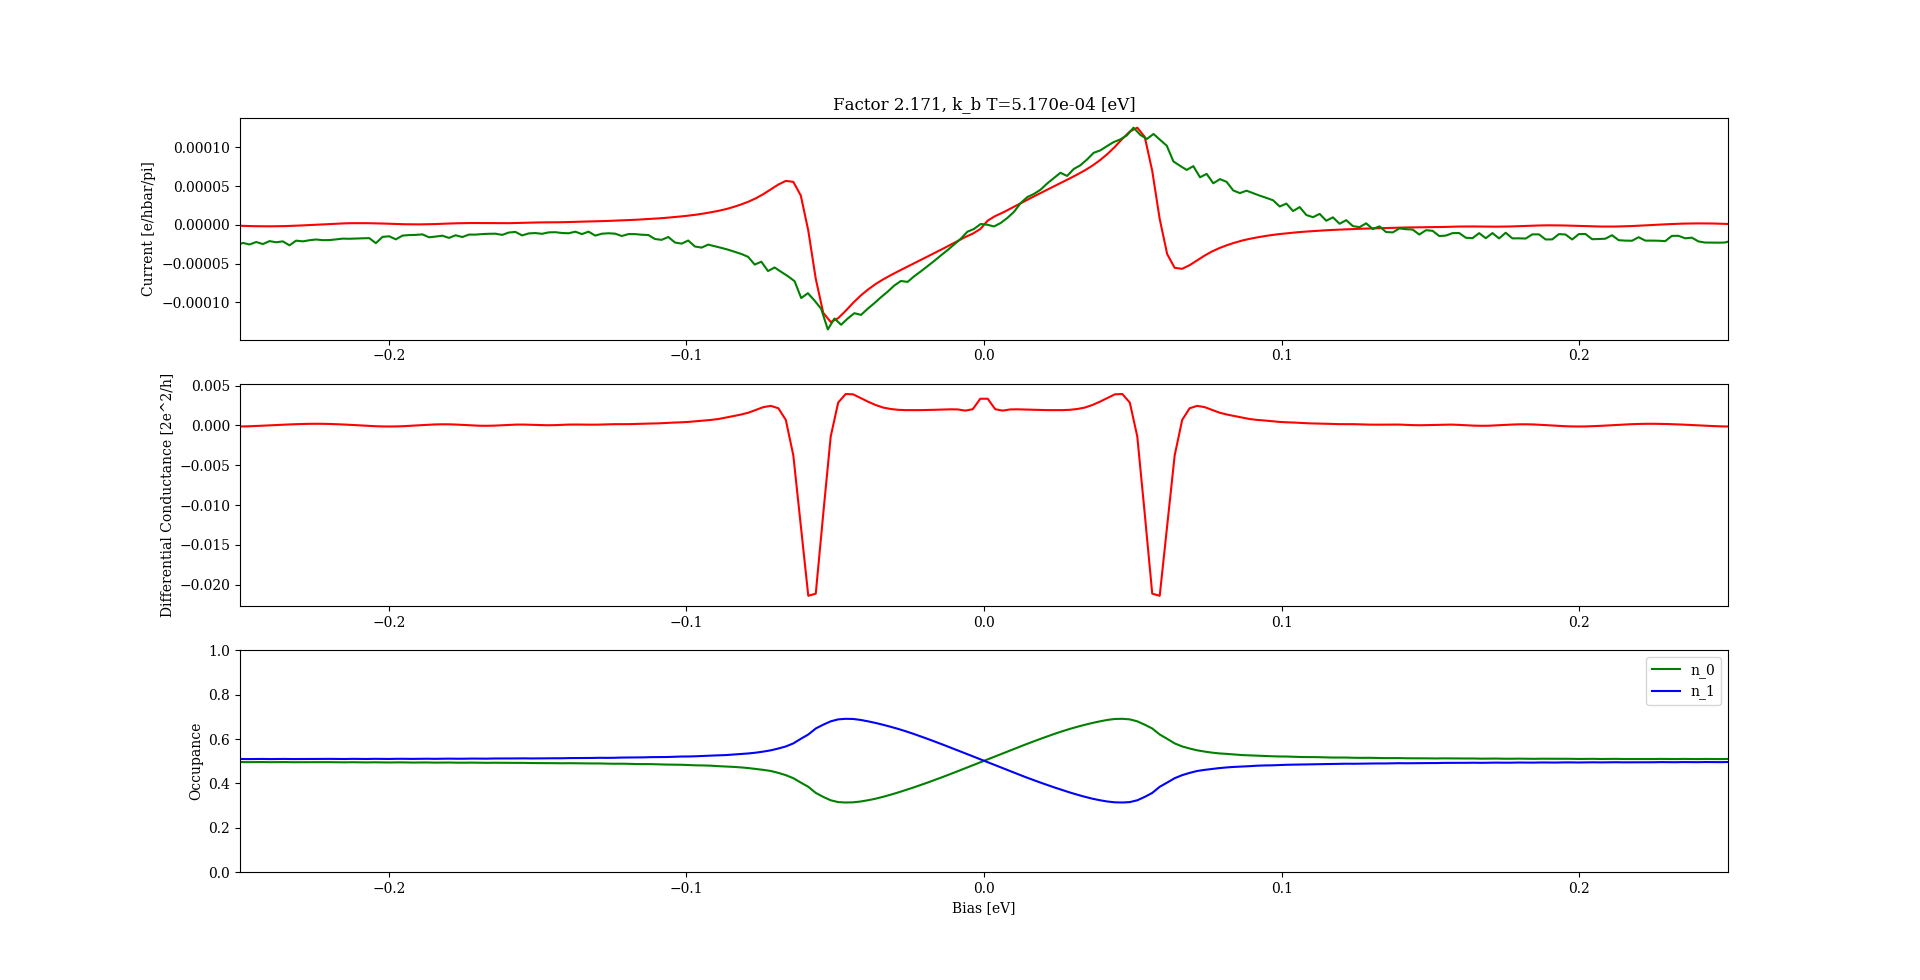
\includegraphics[width=\textwidth]{figure_gam0050alpha55tau024capacitive35points200.png}
        \caption{\label{fig:perrinmolecule} Characteristics of the low-temperature DIH molecule. The calculated current shows great improvement in amplitude and correctly reproduces the NDC features. The drop off after reaching peak current  is faster than found in the experiment (see main text). The differential conductance is nicely symmetric and both show peaks at the predicted value $\pm\sqrt{\frac{4\tau^2}{1-\alpha^2}}$. The occupation of the dot is clearly relevant, as it is fractionally charged at all biases. For this simulation, $k_b T=5.17\cdot 10^{-4}$ eV, $\gamma=0.005$ eV, $\alpha=0.55$, $\tau=0.024$ eV and $U=0.35$ eV.}
    \end{figure*}
    
    \section{Discussion}\label{sec:discussion}
    The authors are extremely awesome.
    \bibliography{references} 
\end{multicols}
\end{document}
